%!TEX root = project.tex

\chapter*{About this project}
\paragraph{Abstract}
This project has been done in conjunction with the Galway Civic Trust. The purpose of the project was to solve the problem the Galway Civic Trust had. The main problem they had was that they had no facility by which the trust could create, read, update and delete walking tours with out the need to have a separate mobile application developed for each tour. 
The system comprises of two main parts a back end web application(Admin Panel) which its self consists of two parts an administration site and an API(Application Programming Interface). The API is protected using jwt and is safe from external injection/attacks. The Admin Panel which is what the trust will use to manage the walking tour's content, has been developed using a MEAN(MongoDB, Express, Angular JS, Node JS) stack approach. The API is used by both the Admin panel and the mobile application to communicate with the database. The second part of the project was to develop a cross platform mobile application that consumes the data from the database, which is provided by the API. The mobile application makes extensive use of Google's Map API for both dynamic and static maps used within the mobile application. The mobile application was developed using the Ionic Framework and Angular JS. 


A brief description of what the project is, in about two-hundred and fifty words.

\paragraph{Authors}
This project has been developed by 3 fourth year students: Arjun Kharel, Trevor Davies and Patryk Piecha for the Bachelors of Science Honours Degree in Software Development.
Arjun was responsible for the back-end web application.
Patryk and Trevor were responsible for the mobile application.

\chapter{Background}
 \cite{galwayTourism} Galway City originally formed from a small fishing village located in the area near the Spanish Arch called ‘The Claddagh’ where the River Corrib meets Galway Bay. Galway later became a walled town in the year 1232 after the territory was captured by the Anglo Normans lead by Richard De Burgo. The town walls, some sections of which can be seen today near the Spanish Arch, were constructed circa 1270. A charter was granted in 1396 by Richard II which transferred governing powers to 14 merchant families, known locally as the 14 tribes of Galway. 
 The 14 tribes relished their independence but retained their close links to the British crown. Galway's strategic coastal location and natural harbour area resulted in a successful trade with both Portugal and Spain and the city prospered for centuries. However in 1651 with the arrival of Cromwell the region entered a long period of decline. Other prominent sea ports emerged on the east coast, namely Dublin and Waterford and trade with Spain came almost at an end. Many years would pass before Galway would again enjoy such prosperity but the legacy of the cities long and colourful history is evident in the character and style of the city. 
 Galway City is a thriving, bohemian, cultural city on the western coast of Ireland. Along with being a popular seaside destination with beautiful beaches and long winding promenade, it also has a buzzing cosmopolitan city centre. The city is a joy to explore with its labyrinthine cobbled streets, colourful shop facades and busy café/ bar culture.  The city is also well known for its many festivals throughout the year with huge crowds gathering for the annual Galway Arts Festival, Races and numerous other events. Old Ireland is present too with turf fires and traditional music featuring in many pubs to compliment your enjoyment of a well-earned pint of Guinness. Take an evening stroll along the promenade and watch the sunset over Galway Bay or watch the salmon fishermen in the River Corrib from the perfect vantage point of the Salmon Weir Bridge.
\cite{galway20} Galway is certainly one of the best tourist attraction in europe because of its rich cultures, traditions, festivals. Galway  and is bidding to become the European Capital of Culture in 2020.The bid represents an opportunity for everyone to join their hands together as a community and reflect and spread the uniqueness of our Galway culture and the richness, vitality and diversity of our shared European culture. \cite{failteireland}Failte Ireland has provided the regional tourism performance of 2014.  The overseas visitor to counties in 2014 shows that, there were total of 1235 people visiting Galway, and ranks 3rd in Ireland after Dublin (4,119) and Cork (1,542). Failte Ireland  has also provided the result of Overseas visitor revenue  (€mn) by county in 2014.  Adapted from : 

\begin{center}    
	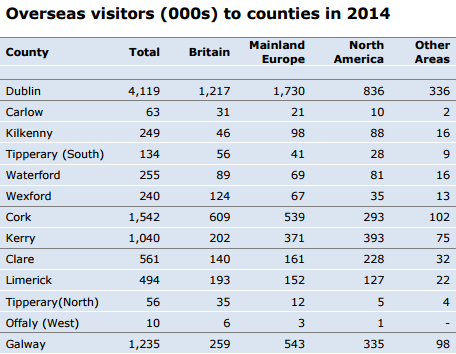
\includegraphics{img/statsgalway.PNG}
\end{center}
\begin{center}    
	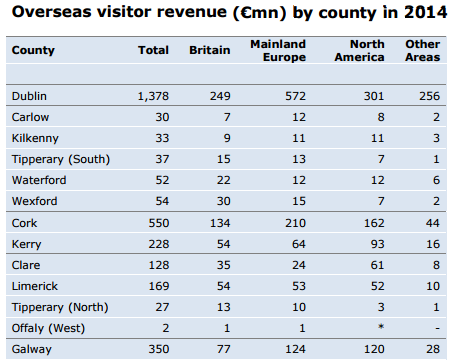
\includegraphics{img/revenue.PNG}
\end{center}



About Galway Civic Trust:  \cite{galwaycivictrust}Dúchas na Gaillimhe - Galway Civic Trust is committed to protecting and enhancing Galway's natural, built and cultural heritage for the benefit of all. The Trust adopts a hands-on approach and undertakes improvement projects which otherwise would not happen. Our offices are located in the Latin Quarter at the Red Earl's Hall archaeological site.
Established in 1992, we have completed over 50 projects, ranging from the erection of historic wall plaques to the refurbishment of Rusheen Bay Bird Sanctuary and restoration of the Fishery Tower at Wolfe Tone Bridge.
In partnership with the Department of Social Protection, Galway City Council and Galway County Council, Galway Chamber of Commerce and Industry, The Heritage Council of Ireland, and the local community, we undertake works for the enhancement of Galway city and county.

\chapter{Introduction and Context}
	\section {General Problem Statement}
	A facility the Galway Civic Trust provides is arranging walking tours in and around Galway City. The trust came to the college this year to address a major problem they had with the current walking tour mobile applications they had. The problem they had was that currently there was no means by which to create,update or delete any information with in the mobile applications they had already. This meant that every time they created to new walking tour, it necessitated the creation of a new mobile application being developed for that specific tour. This current system is very impractical and required the constant creation of new mobile applications.
		
	Therefore our two main tasks/objectives for this project were to develop for the Galway Civic Trust an integrated back end(Admin Panel) that the trust would use for content management of their walking tours and a cross platform mobile application that would dynamically consume the tour content through an API. The trust can perform CRUD(create,read,update and delete) operations through the use of the Admin Panel. These operations will be synchronised across all the consuming devices/mobile applications via the API.
	
	The goals and objectives of developing this system for the Galway Civic Trust, is to allow for instantaneous synchronisation of the database and the consuming devices through an API so that the data can be received in real time. The development of such an application will differently solve the problem for the Galway Civic Trust. This application will eliminate the need for time consuming visits to GMIT, and enable the Galway Civic Trust to effectively and efficiently make any adjustments to existing tours or create new tours in the cross platform mobile application through the use of the Admin Panel web application.
	
	\section {Previous work}
	In previous years the Galway Civic Trust approached GMIT in order to create Walking Tour mobile applications for them. There were two applications made. One using the Ionic Framework and  Angular JS, the second was completed using Phonegap and the jQuery Mobile Framework. A major draw back to these applications is the fact that they both use static data contained with in the application. This meant that the trust had no way of preforming any adjustments to the applications. Nor could they add more tours to them.
	
	\section {Purpose}
	The whole purpose of this project is to develop a system that facilitates the need the trust had to be able to create tours without the need to have a separate Mobile application developed for each tour. Secondly to have a cross platform mobile application to consume the data content. We have aimed to achieve this by creating a system that enables the trust to perform all the necessary tasks involved in the creation and maintenance of the walking tours, and to produce a mobile application that consumes this data. We believe the system that has been created achieves this task. The Admin Portal web application provides all necessary functionality to enable the Galway Civic Trust to create/maintain the tours that they have created, and the Ionic cross platform mobile application is able to display the tours through static data and dynamic data.
	
	\section {Scope Objective and Goals}
	This project has been separated into three uniquely different independent parts that all communicate with each other. 
	\begin{enumerate}
		\item{The Back-end (Admin Panel): Used by Galway Civic Trust to manage and maintain all existing tours and create new tours through the use of a graphical and interactive user interface. Different user roles have been added these include admins, Super Admins. Super Admins have permission to manage/add new admin accounts whereas regular admins don’t.}
		\item{RESTful API: Used by both the Admin Panel and the Ionic App and allows mobile devices to consume the JSON data. Changes made in the database can in real-time be consumed by devices through the use of the API}
		\item{Ionic Mobile App: Cross platform hybrid mobile app has been developed using Ionic framework. The mobile application pulls the data through its communication with the API.}
	\end{enumerate}
	
	 Objective and Goals: Our objectives and goals stems from projects/systems previously completed by former students of Software Development Course in GMIT. Our main objective and goal is to solve the problem stated in the problem statement. Our main goals and objectives of this project are as follows:
	 \begin{itemize}
		\item Develop Back-end for tour content management.
		\item Develop Restful API so that the client application can consume data in real time. 
		\item Cross platform hybrid mobile application for consuming the API.
		\item Google Maps navigation and direction services.
		\item Instant synchronization of data  between API consuming devices and backend. 
	\end{itemize}
	\section {Roadmap}
	So, at this point, we have discussed about what the project is, and the reason for taking this project. Now, let me explain few sections/chapters of this review briefly so you will have a better understanding of a project.
	Methodology  - This section provides the development methodologies we used to develop this project, including project meetings, collaboration tools used, interaction with the client and weekly meeting with the project supervisor. 
	Technology review : This section provides the research that was carried out when choosing the technology . This section also provides the selection criteria and the particular reason for choosing the specific technology.
	System Design : This section gives detailed information about actual system, and the way it is functioning. This section also talks about the architecture of a project, Data models, use cases etc.  
	System Evaluation : This section provides evaluates the system based on the following attributes.
	Scalability
	Robustness
	Maintainability
	Extensibility 
	Reliability 
	
	Conclusion and Recommendation: This section summarises the context of a project, objectives and goal achieved. 
	We have talked about different sections of this project briefly and now I would like  to include the resources url of this project.  Due to the nature of this project, we have created three different repositories in Github as because they were developed independently of one another and at the end they are talking using the middleware technologies and different protocols. This is explained in detail in the technology review section.  Following are the repositories in the github.
	

\chapter{Methodology}

The process of deciding which technologies to use was done after the initial meeting with the Galway Civic Trust. After receiving the objectives and goals for the project we started to research which technologies and processes would be best suited for the project based on these objectives and goals. As we were not given a list of requirements our first task in developing this system was to decide on a list of requirements. Firstly we discussed the back-end web application that would be developed to achieve the main objective which was to create a means by which the Galway Civic Trust could create and maintain data relating to the creation of walking tours. At our first meeting it was decided that a NoSQL Database would be best for storing the date required for the back-end. Because MongoDB had been used before hand in a previous project it was decided that we would use it as the database for the project and that the whole back-end system would adapt a MEAN stack approach. A RESTful API would be used as the middleware, which would sit in-between the database and the Mobile application.  At this point we discussed what type of Mobile application would be developed to consume the data within the database which would be provided by the API.

A cross platform mobile development framework for the mobile application was decided to be the best route to take when developing the end-user product and so we chose to use Ionic Mobile Framework. At this point we created a project plan using Microsoft Project to assign different tasks. Because the project had been divided into three different parts we created three separate Github repositories, one for the back-end, one for the Ionic Application and one for documentation. 
\begin{itemize}
	\item{(Back-End)https://github.com/ultimatecodelab/Galway-Civic-Trust.git}
	\item{(Ionic Mobile Application)https://github.com/TrevorDavies/Galway-Civic-Trust.git}
	\item{(Documentation)https://github.com/Paddero/GCT-Documentation.git}
\end{itemize}

We used Agile software development methodology for this project because of the projects nature. The requirement was not clearly specified to us and therefore, we had to develop the system in an incremental way. We had a weekly project meeting with our project supervisor Damien Costello. Mr. Damien Costello helped to guiding us throughout the entire development of this project. Every week/fortnight  our work was presented to our project supervisor and feedback was received.  As the development group consisted of three members, we had two-three meetings per week to discuss how we were getting on with  the project. We also created the facebook group chat for interaction outside the college. 


Testing: Talk about Selenium Webdriver here.... Attach few test cases...


\chapter{Technology Review}
	In this section we are going to talk about the technology used in this project.  We have used various types of new technologies. This sections will cover about the technology choices and the reason for choosing the technologies. We have used MEAN stack for backend development, Ionic Framework for cross platform app development and JustInMind as a prototyping tool.  We are first going to talk about prototyping tool then MEAN stack and finally we will look at the ionic framework and cross platform development. 

	\section{Prototyping Tool - Justin-mind}
	 JustInMind  in All-In-One prototyping tool for web and mobile app. \cite{JustInMind} It allows you to to provide prototype faster and better with default built-in widgets. These widgets have been specifically designed to fit our IOS or Android app, so you content always looks great.  JustInMind also provide the web framework to prototype web applications. Every widget in web framework is designed to help your web wireframes. JustInMind includes handy collection of web buttons, menus, charts  and more that can be used automatically.  JustInMind also gives us an ability to embed HTML and Documents. The widget library allows you to insert HTML, Docs and video, including online widgets, interactive maps and other on/offline content, to name a few. 
	 
	\section{MEAN-Stack}
	So, what exactly is MEAN stack ?Well, in nutshell \cite{Mean-Stack} MEAN is a free and open-source JavaScript software stack for building dynamic web sites and web applications. The MEAN stack makes use of MongoDB, Express.js , Angular.js and Node.js. Because all components of MEAN stack support programs written in JavaScript, MEAN applications can be written in one language for both server-side and  client-side execution environments. In order to fully understand the use and why MEAN stack is so popular and one of the mostly used javascript software stack, we must talk about its components. Let's start with M (MongoDB) of MEAN stack.
	
		\subsection{NoSql Technology - MongoDB}
		MEAN stack comes with a NoSql database technology called MongoDB. Before talking about MongoDB itself it is important that we understand what NoSql technology is about. \cite{NoSqlTechnology}  Not only Sequential Query Language(NoSql) is a database that provides a mechanism for storage and retrieval of data which is modeled in means other than the tabular relations used in relational databases. NoSql databases have been proven to be the solution to what is known as Big Data as they follow a schema-less data model, hence provide increased scalability and flexibility as compared to relational databases. In recent years, developers and organization have experiences a sharp rise in volume of user data and products that has to be stored in databases \cite{MongoOfficial}. NoSQL databases are widely used to store and retrieve very large amounts of data using a key-value format \cite{VeronikaAbramova}. These types of databases have emerged as the best choices that suite modern mobile and web development.
		We discussed briefly about the NoSql database technology. Now let's briefly talk about MongoDB .
		
		MongoDB : This is a document store, non-relational, open-source database developed by 10gen. The name mongo is extracted from the word humongous. It provides high availability , high performance, and automatic scaling and allows data insertion without a predefined schema. A record in MongoDb is composed of field and value pairs and are predefined schema. A record in MongoDb is composed of field and value pairs and are similar to JSON objects. The value of field may consists of arrays, and array of documents or other documents. MongoDb maintains data consistency in the sense that one write operation to the data in the database allow subsequent read operation. They use a locking mechanism that contributes to increased execution time as the number of update operation increases. \cite{MongoOfficial} \cite{EricRedmond}.
		
		
		Anam Zahid , Rahat Masood , Muhammad Awais Shibli, in their paper describe how MongoDb  offers horizontal scale-out  for databases using a technique called sharding. With sharding, a data is distributed across multiple physical partitions known as shards. This was designed in order to address the hardware limitations where only a single server existed and contributed to such things as bottlenecks in RAM or disk I/O. MongoDB has the sharding functionality automatically built into the databases and the size of the data grows, MongoDb automatically balances the data in the shard and so when the size of cluster decreases or increases. As a result , a dynamically balanced load is experienced. Concurrency control measure for multiple clients accessing the same database are enforced by mongoDB by managing multi-threaded access to shared objects and data structures. \cite{MongoOfficial} \cite{MongoDbArchitectureGuide}.
		
		
		
		\subsection{Express.js}
		\cite{expressRef}Express.js is another component of MEAN Stack. Express is a nodejs based web framework, inspired by Sinatra and it is asynchronous. Express.js builds on the underlying capability of Node, by providing a web application server framework. Express.js is a Node.js web application server framework, designed for building single-page, multi page and cross platform hybrid web applications\cite{expressRefWiki}. 
		
		\subsection{Node.js}
		Node.js is a Javascript runtime built on Chrome’s V8 JavaScript Engine. Node.js uses an event driven, non-blocking I/O model that makes it lightweight and efficient web server environment, idea for constructing a web-service API’s\cite{Node.jsWiki}. Node.js package ecosystem, npm, is the largest ecosystem of open source libraries in the world. \cite{expressRefWiki} 
		
		\subsection{AngularJs}
		The last component of a stack is Angularjs. The official documentation \cite{Angularjs}defines angularjs as - AngularJS is a structural framework for dynamic web apps. It lets you use HTML as your template language and lets you extend HTML's syntax to express your application's components clearly and succinctly. Angular's data binding and dependency injection eliminate much of the code you currently have to write. And it all happens within the browser, making it an ideal partner with any server technology.
		
		Angularjs provides client-side framework for MVC  \cite{Angularjs} single page web application. To take full benefit of Angular, it can be well be used with other software packages like Yeoman and Bootstrap. Yomean provides an environment which enables the use of generators: simple script-based tools that can be used to scaffold the bare-boles of  Angular web app. \cite{YeomanGenerator}.  There are several reason why angularjs is so popular and few reasons includes: 
		
		1: As mentioned above, Angularjs structure the source code by following the Model View Controller. 
		2: Another power feature of Angularjs is the capability of two way data binding. It lessens the amount of boilerplate code which is written to keep the model and view in agreement.
		3:  Angularjs models are plain old java object (POJO), therefore it is simple to change or append properties without any complications.
		4 : Another most important feature of Angularjs js is about dependency injection. Dependency injection is a software design pattern that deals with how components get hold of their dependencies. The angular injector subsystem is in the charge of creating components  resolving their dependencies, and providing them to other components as requested \cite{AngularJSDi}. 
		So, we spoke about the main components of MEAN stack briefly and  now you should have better understanding  of this technology.  Lets us now talk about the RESTful api that as been developed for the consumption of our data by the mobile device(end user).
		
		\section{REST- Architecture}
		\cite{expressRefWiki}\cite{restProgramming} Representation State Transfer, widely knows as the REST or RESTful model for web-services, uses the native HTTP operation: POST,GET,PUT, and DELETE to map on to the four fundamental database operations. - Create,READ,UPDATE,DELETE. API can be built to link these four HTTP verbs to functions which Create, Read, Delete or Update records within a web-services. This service can be consumed by any time of authenticated client device. 
		
		\section{Passport JWT - JSON Web Tokens Authentication}
		The backend(admin portal) and the API is fully protected using JSON web tokens. System user Login and API endpoints has been all protected from external injection.  \cite{AnatomyOfJWT} \cite{IETFRFC} \cite{DraftIETAOAUTH} [19,20,21] JSON web tokens are open, industry standard RFC 7519 method for representing claims securely between two parties.  Token based authentication is prominent everywhere on the web nowadays. With most every web company using an API, tokens are the best way to handle authentication for multiple user. JWT is separated into three parts, Header, Payload,  Signature.
		
		 Header: The header contains two parts - declaring the type, which is jwt and the hashing algorithm to use (HMAC SHA256 )
		 {
		 	“Typ”: ”JWT”
		 	“Alg”: ”HS256”
		 }
		 2: Claims :  The payload will carry the bulk of our JWT, also called the JWT claims\cite{AnatomyOfJWT}. This is where we put the information that we want to transmit and other information about our token. The claims contains any information that you want signed\cite{StormpathJWT}.
		 3: JSON web Signature: The headers are claims digitally signed using the algorithms in the specified in the header.  The header and claims are JSON that are base64 encoded for transport. The header, claims, and signature are appended together with a period character \cite{IETFRFC}
		 \cite{DraftIETAOAUTH}. \textbf{The JWT authencation is handelled using passport module that is available from npm. This module lets you authenticate endpoints using a JSON web token. It is intended to be used to secure RESTful endpoints without sessions.}
		 
		 
	\cite{HyphemeJWT} One great advantage of tokens is that we don't have to lookup the token in a database on every api call as it contains all needed information in itself. This should help keeping the authentication process small. The biggest downside of that is the inability of revoking a token without having a whitelist or blacklist somewhere. This is the reason we keep the lifetime of the token small (120 minutes in this example)
		 
 Here is  an example configuration which reads the JWT from the http Authorization header with the scheme 'JWT' \cite{JWTPassport}:
		 
\begin{minted}{js}
	 var JwtStrategy = require('passport-jwt').Strategy,
	 ExtractJwt = require('passport-jwt').ExtractJwt;
	 var opts = {}
	 opts.jwtFromRequest = ExtractJwt.fromAuthHeader();
	 opts.secretOrKey = 'secret';
	 opts.issuer = "accounts.examplesoft.com";
	 opts.audience = "yoursite.net";
	 passport.use(new JwtStrategy(opts, function(jwt_payload, done) {
	 User.findOne({id: jwt_payload.sub}, function(err, user) {
		 
	 if (err) {
	 return done(err, false);
	 }
	 if (user) {
	 done(null, user);
	 } else {
	 done(null, false);
	 // or you could create a new account 
			}
	});
	}));
		 
\end{minted}

		
		\section{Send-grid - Email Delivery}
		 The  process of sending email to system admin with instructions to reset the password has been achieved using SendGrid API. SendGrid provides a cloud-based email delivery service that assists business with transactional email management \cite{sendGrid}. SendGrid is chosen in this project for password recovery email delivery service because it is very reliable and have advanced spam filtering system. We got sendgrid for absolute no cost for development purpose. 
		 
		\section{Cross-Platform Development}
		End user mobile app has been developed in Ionic Framework.  The requirement of this project was to target at least two major platform, Android and IOS. Ionic framework was was a perfect choice for us because It is free and open source, Ionic offers a library of mobile-optimised HTML, CSS, and JS CSS components, gestures, tools for building highly interactive apps. Built with Sass and optimised for AngularJs \cite{expressRef}.
		
		\section{Google Maps}
		For GPS navigation and directions of a tour in consumer (ionic app), google Direction service is used. It allows you to calculate directions by using the DirectionsService Object. Adapted from \cite{GoogleMapDirection}, the official documentation .This object communicates with the Google Maps API Directions Service which receives direction requests and return computed results. You may either handle these directions results yourself or use the DirectionsRenderer object to render these results. 
		
	
About seven to ten pages.
\begin{itemize}
	\item Describe each of the technologies you used at a conceptual level. Standards, Database Model (e.g. MongoDB, CouchDB), XMl, WSDL, JSON, JAXP.
	\item Use references (IEEE format, e.g. [1]), Books, Papers, URLs (timestamp) – sources should be authoritative. 
\end{itemize}



\chapter{System Design, Implementation and Deployment}
As many pages as needed.
	\section {System prototype}
	Prototyping tools used : Reasonable amount of time was spent initially in the design phase of this application . We have designed our both backend (Admin portal ) and Ionic mobile app using , one of the most popular prototyping software called JustInMind Prototyper. 
	
	\section{Architecture}
	Architecture : The application is separated into three layers.  Presentation layer, Business logic layer and Data access layer.
	\begin{center}    
		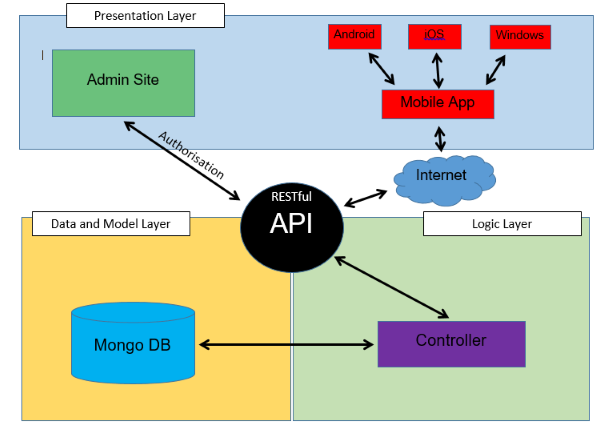
\includegraphics{img/architecture.PNG}
	\end{center}
		\subsection{Presentation Layer}
		 In presentation layer you can see the Admin Site (Admin portal) ,this is a graphical user interface where system admin can manage the contents and accounts of the users registered.  On the right hand side, you can see many mobile devices of different platform consuming the data from API. Consuming app is only allowed to send GET request to API because all we care in end user app is being able to retrieve the data dynamically loaded from the api. On the admin portal, any CRUD operations needed to perform requires authorization and authentication of registered admin. The user interface in presentation layer was developed in angularjs and Ionic framework. The main components of presentation layer are as follows : In this layer will will discuss about the admin portal user interface and end user mobile apps user interface. 
		
		 	\begin {center}    
		 		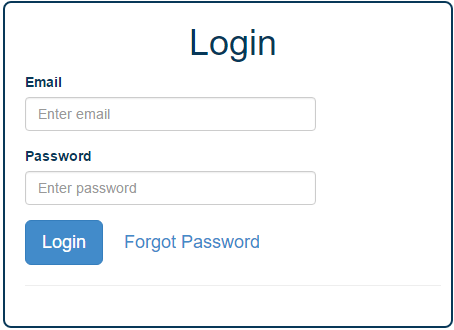
\includegraphics{img/gctloginpage.PNG}
		 	\end{center}
		 	Login screen for system admin. If admin forgot his password, it can easily be reset using forgot password link . The system will check and verify that the specified admin exist in the database and it exists, system will generate a random temporary password and send and email. 
		 	
		 		\begin{center}    
		 			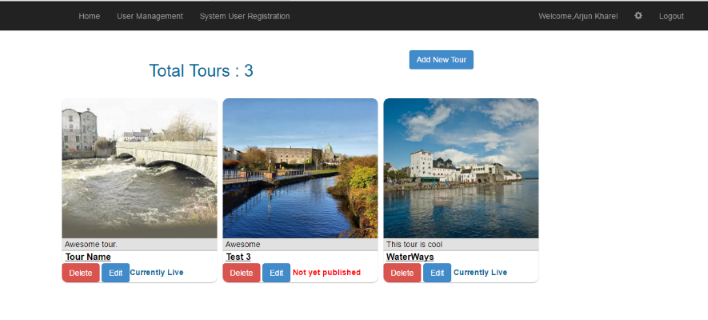
\includegraphics{img/MainPage.PNG}
		 		\end{center}
		 		This is the landing page of admin panel. When admin logs into the website successfully they will then be brought to this main page where they can see all the tours they have published. The tour also represent its state, ie. published or Not yet published. Admin can easily from CRUD operations. 
		 		
		 		LOCATION page
		 		\begin{center}    
		 			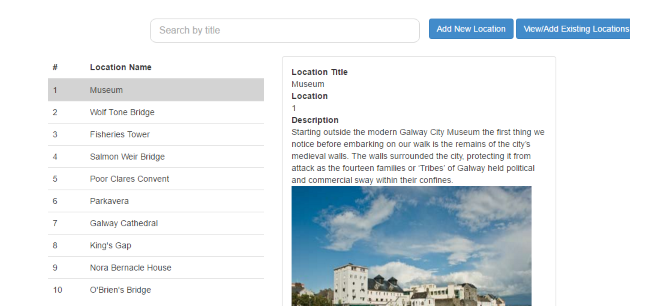
\includegraphics{img/locationPage.PNG}
		 		\end{center}
		 		When you click on the tour in the main page, you will be brought to this (location page) where you can see all the locations/walks within that tour.System admin can perform CRUD operations. 
		 		 	USER MANAGEMENT PAGE
		 			\begin{center}    
		 				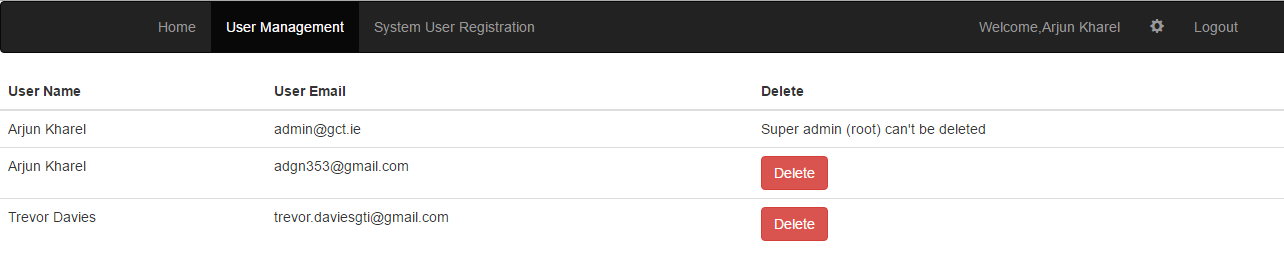
\includegraphics{img/userManagement.PNG}
		 			\end{center}
		 		
		 			This is one of the powerful feature of this project. This is a user management section.  Remember, there are two types of admin roles in this project. Super admin and Regular admin. If you are logged in as a superuser then you will have access to user management, system user registration pages.
		 			
		 			\begin{center}    
		 				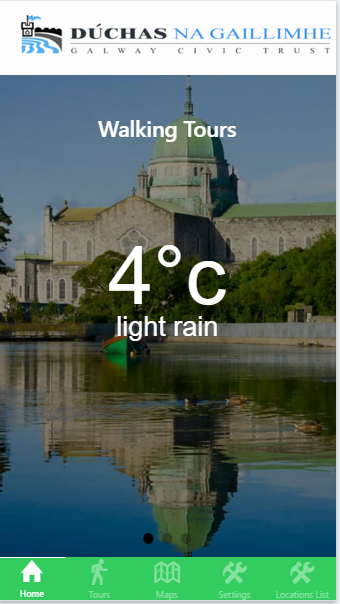
\includegraphics{img/ionicmanepage.PNG}
		 			\end{center}
		 			This is the landing page of the mobile application. The application is very clean and attractive. It shows the weather and on the bottom it have different tabs for navigation purpose. 
		 			
		 				\begin{center}    
		 					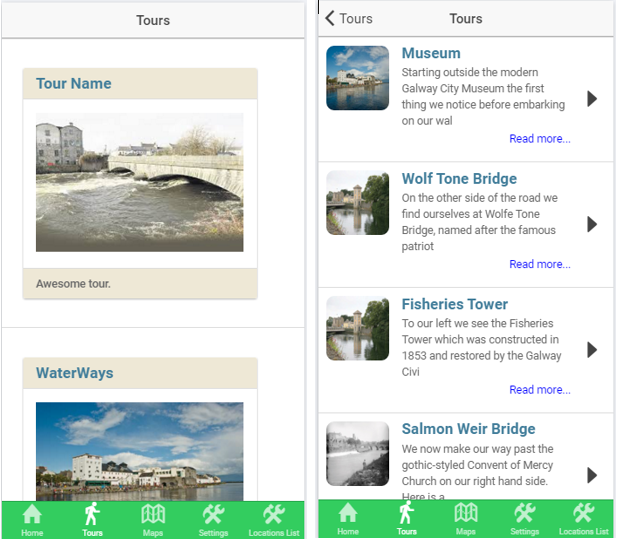
\includegraphics{img/toursandlocations.PNG}
		 				\end{center}
		 				When user clicks on the tours, they will be brought to the page on the left. End user can see all the tours available. When they click on a tour, they will be brought to the location page where it displays all the location or walks in that tour. 
		\subsection{Business Logic }
		We have talked about the presentation layer of this application . Now let's talk about the business logic layer and how everything is connected.  The business logic has been written in javascript. Every functionality has its own controller.  When consumer app send the GET request to an API endpoint, appropriate controller is called to complete the request. The thing to remember here is, external user / external request is not directly connected to our database. The controller is used to retrieve the information from the database and response is sent back to the browser. There is no direct connection to the database therefore any request coming is handled by an API and controllers working together.  Please refer to the architecture diagram above for better understanding of this process. 
		API route and appropriate controller is invoked to complete the request. 
		
		How tour is uploaded in the database ?
		1: Angularjs Controller
		2: Send post request to backend API
		3 : API  now insert data in mongodb..
		
		
		1: AngularJs upload tour controller :
		
\begin{minted}{js}
	 $scope.uploadTour = function(file) {
	 console.log($scope.tour);
	 Upload.upload({
	 url: '/api/tour/upload',
	 headers: {
	 'Content-Type': 'multipart/form-data'
	 },
	 data: {
	 file: file,
	 title: $scope.tour.title,
	 description: $scope.tour.description,
	 status:$scope.tour.status,
	 _creator: $scope.user._id
	 }
	 }).then(function(resp) {
	 alertSuccess.show();
	 console.log('success ' + resp.config.data.file.name + 'uploaded. Response: ' + resp.data);
	 $scope.tours.splice(0, 0, resp.data);
	 $scope.tour.title = '';
	 $scope.picFile = '';
	 $scope.picPreview = false;
	 alertSuccess.show();
	 
	 }, function(resp) {
	 
	 alertFail.show();
	 }, function(evt) {
	 var progressPercentage = parseInt(100.0 * evt.loaded / evt.total);
	 console.log('progress: ' + progressPercentage + '% ' + evt.config.data.file.name);
	 });
	 
	 }//uploadtours
	 toursAPI.getAllTours();
	 }
\end{minted}
		
		
		
		
		
	   \begin{minted}{js}
 exports.upload = function(req, res) {
	 var newTour = new Tour();
	 var fileimage = req.middlewareStorage.fileimage;
	 
	 console.log("The description is :"+ req.body.description);
	 newTour.image = '/assets/images/uploads/' + fileimage;
	 newTour.title = req.body.title;
	 newTour.description = req.body.description;
	 newTour.status = req.body.status;
	 newTour.createTime = Date.now();
	 
	 newTour.save(function(err, tour) {
	 if(err) {
		 console.log('error saving tour');
		 return res.send(500);
	 } else {
		 console.log(tour);
		 res.status(200)
		 .send(tour);
		 }
	 });
 };
	   \end{minted}
 POST and PUT routes protected
 
 \begin{minted}{js}
 router.post('/upload', auth.isAuthenticated(), controller.upload);
 router.post('/updateTour', auth.isAuthenticated(), controller.updateTour);
 router.post('/updateCurrentLocation', auth.isAuthenticated(), 
 router.post('/uploadLocation', auth.isAuthenticated()
 \end{minted}
	
Controller to receive all the locations of a specific tour and sorting by timestamp to determine the order of the tour inserted

\begin{minted}{js}
	exports.getAllPublishedTours = function(req, res) {
		Tour.find({status:true})
		.sort({
		createTime: -1
		})
		.exec(function(err, tours) {
		if (err) {
		return handleError(res, err);
		}
		if (!tours) {
			return res.send(404);
		}
		console.log(tours);
		return res.status(200)
		.json(tours);
		});
	};
\end{minted}
		\subsection{Data Layer}
			Mongoose Models - MongoDB
		\begin {center}    
		\includegraphics{img/dataModels.PNG}
		\end{center}
		The back-end comprises of 3 collections. Locations , Tour and Admin collection. The model is represented as a mongoose model. Mongoose provides a straight-forward, schema-based solution to model your application data. It includes built-in type casting, validation, query building, business logic hooks and more, out of the box. Lets talk about the each of  field in the collections (models) and about their purpose. 
		
		\textbf	{Location:} - Lets us talk about the important field in the location collection. Location ID : is a unique ID assigned by MongoDb, TourID is an array that contains the ID of the tour. This is very important in this project because it is used to identify the location-tour relationship or in another words, to find out which tour the particular location belongs to. Data structure is Array because a location can be shared in one or many tours and we don't want to replicate the same data more than once. By having Tour ID array, we can keep track of the location and in how many tours it is being shared.
		The Shared Counter is another field that determine, how many tours is currently using that location. This is useful when we want to share the location is multiple tour. 
		
		Location model representation in Mongoose:
	\begin{minted}{js}
	var mongoose = require('mongoose');
	var Schema = mongoose.Schema;
	
	var LocationSchema = new Schema({
	image: String,
	title: String,
	tourId : String,
	tourIdArr : [String],
	sharedCounter:Number,
	description: String,
	location: String,
	xCoordinate: String,
	yCoordinate: String,
	_creator: {
	type: Schema.ObjectId,
	ref: 'User'
	},
	createTime: {
	type: Date,
	'default': Date.now
	}
	});
	
	module.exports = mongoose.model('LocationSchema', LocationSchema);
		
	\end{minted}
		
		\textbf	{Tour:} - Tour collections contains basic information about a tour.  Title represent a tour title, status identifies if  the tour is currently published or still under the development. Only with the status "published" tours are synchronised to the consuming devices. 
		
		Tour model in mongoose
		\begin{minted}{js}
	var mongoose = require('mongoose');
	var Schema = mongoose.Schema;
	
	var TourSchema = new Schema({
	image: String,
	title: String,
	description:String,
	status: Boolean,'default':false,
	createTime: {
	type: Date,
	'default': Date.now
	}
	});
	
	module.exports = mongoose.model('Tour', TourSchema);
	\end{minted}
	
		
		\textbf{Admin:} - This collection is the admin collection. This contains the details of system admins. The model of this collection in mongoose looks like this. 
		
	\begin{minted}{js}
	var mongoose = require('mongoose');
	var Schema = mongoose.Schema;
	var crypto = require('crypto');
	var UserSchema = new Schema({
		name: String,  
		email: {
			type: String,
			lowercase: true
		},
		role: {
			type: String,
			default: 'user'
		},
		hashedPassword: String, //hashed password
		provider: String, //authencation provider
		salt: String
	});
	\end{minted}
		
\section{Deployment - Digital Ocean}
	Digital Ocean is a provider of Virtual Private Servers (VPS) that all run over the internet. Their claim to fame is the speed of their images (they were one of the first, if not the first, providers to offer SSD images) and their assertion that it only takes 55 seconds to setup an SSD cloud server. Once you get through the initial account setup process (username and password, billing setup) this isn’t too far off from reality.  Digital ocean is very straight forward to deploy your application and very simpler other cloud hosting provider like Amazon Aws , Azure and Heroku. We also a free digital ocean subscription from GitHub student pack and we used it throughout the development of backend. 
	
	Instruction to deploy on cloud server:
	please follow this link here, official digital ocean instructions for deploying a nodejs app for production.
	
	https://www.digitalocean.com/community/tutorials/how-to-set-up-a-node-js-application-for-production-on-ubuntu-14-04


\chapter{System Evaluation}

	The problem we were trying to solve that is mentioned in the problem statement of introduction section is solved. Back-end is fully functional and tested using WebDriver java.We have successfully implemented what we initially wanted to do. Back-end (Admin Portal) is the hardest part of this application development, and the reason is, all the content management, authentications, and API creations is done in the back-end side of this system. The end user app built in ionic framework  is simply consuming the data from an API,and the synchronization is very quick and is working effectively. 
	
	In this section we are going to evaluate our system based on different attributes. They are as follows : 
	\begin{itemize}
	\item	Scalability
	\item	Robustness
	\item	Maintainability
	\item	Extensibility 
	\end{itemize}
	
    \textbf{Scalability: } :  The system is highly scalable when the requirement grows or the data in the database increases in the near future. MongoDb is used to store the datasets and it is widely used in the Industry. NoSql database technology and scalability issues is resolved easily. 
    
     \textbf{Robustness: } The system is very robust and works without any issues.
     The system has been tested in Selenium Webdriver. Various test has been conducted to check the strength of the system. Test cases are available in the github project. The routes/endpoints in the backend are fully protected from any external injection, using the JWT - passport. 
     
     
    \textbf{Maintainability} - This documentation provide clear understanding of the project. Future maintenance should not be a problem because it is very well structured. Model view Controller patterns was used throughout the development and everything is well structured in cohesive manner. The code is highly documented and it does't not impose future maintenance issues.
    
    \textbf{Extensibility} - The development of API makes it possible for many applications to consume the data. If Galway Civic Trust want to use the tour information in different project/system, they do not have to create or insert the same data in another application . The data can be easily shared using the API we built in this project for the consumption by mobile devices.
    Lets say, if GCT want to add one more feature in the future, developer can easily insert a route code a controller to do that specific task. There is absolutely no need and will never have to mock around with other functionality to implement a new feature. No technical debt has to be paid back to add new functionality because the project was developed by adapting various software design principles and design patterns. 
    
	\section{Testing}
	We do believe our system is robust because we have tested all the functionality throughout the development process. We used Selenium Web-driver to test the admin portal. We have tested all the core functionality using Junit (Web-driver), tested browser compatibility and Ionic App has been tested in many different mobile devices. All the Junit test cases are available in the Git-Hub repository. Both Admin Panel (Backend)  and the Ionic App is free of bugs, and run very smoothly.  The chances of crashing is very unlikely, unless there is a fault in the hardware itself.  
	
	
\begin{itemize}
	\item Prove that your software is robust. How? Testing etc. 
	\item Use performance benchmarks (space and time) if algorithmic.
	\item Measure the outcomes / outputs of your system / software against the objectives from the Introduction.
	\item Highlight any limitations or opportuni-ties in your approach or technologies used.
\end{itemize}

\chapter{Conclusion}
About three pages. WRITE YOUR CONCUSION HERE...

\begin{itemize}
	\item Briefly summarise your context and ob-jectives (a few lines).
	\item Highlight your findings from the evalua-tion section / chapter and any opportuni-ties identified.
\end{itemize}
